\documentclass{article}
\usepackage[utf8]{inputenc}
\usepackage{amsmath}
\usepackage{amsfonts}
\usepackage{graphicx}

\title{Discussion Assignment Unit 3\\
Math 1201- College Algebra.
}
\author{Instructor - Casmir Onyeneke}
\date{September 2021}


\begin{document}

\maketitle

\section*{POLYNOMIAL FUNCTION}
For this discussion assignment I would be focusing on the construction sector and the question goes like this\\
“An open box is to be constructed by cutting out square corners of x-inch sides from a piece of cardboard 8 inches by 8 inches and then folding up the sides. Express the volume of the box as a function of x” (Abramson, 2017, p374)\\
\\\title \textbf{Solution}
The question requires that we express the volume of a box as a function of square corners of x-inch sides that were removed from a piece of cardboard from which the box is constructed from.

The volume of any given box is given as $${v = l.w.h}$$
The image is shown below(Chegg.Com, 2016)\\
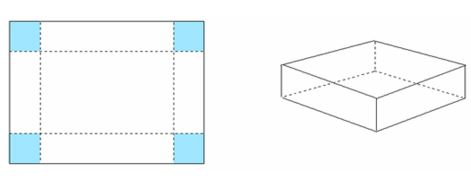
\includegraphics[scale = 0.5]{box}

The sides in blue are the square corners of x-inches.\\
These are the dimensions of the cardboard ${l = 8 inches, \quad w = 8 inches}$

Now the sides of the Newly constructed box can be expressed in terms of the square corners of x-inches.\\
$${boxLength = 8 -x -x}$$
$${boxWidth = 8 -x -x}$$
$${boxHeight = x}$$

So we can therefore express the Volume which is given as  ${v = l.w.h}$ as a function of the square corners of x-inches.\\
$${V(x) = (8-2x)(8-2x)x}$$
Expanding the polynomials 
$${V(x) =(64-16x-16x+4x^2)x}$$
$${V(x) =(64-32x+4x^2)x}$$
$${V(x) =64x-32x^2+4x^3}$$

So therefore the function
$${V(x) =64x-32x^2+4x^3}$$
Expressess the volume of the box as a function of the square corners of x-inches gotten from the cardboard.\\
\\The graph of this function is shown below.\\
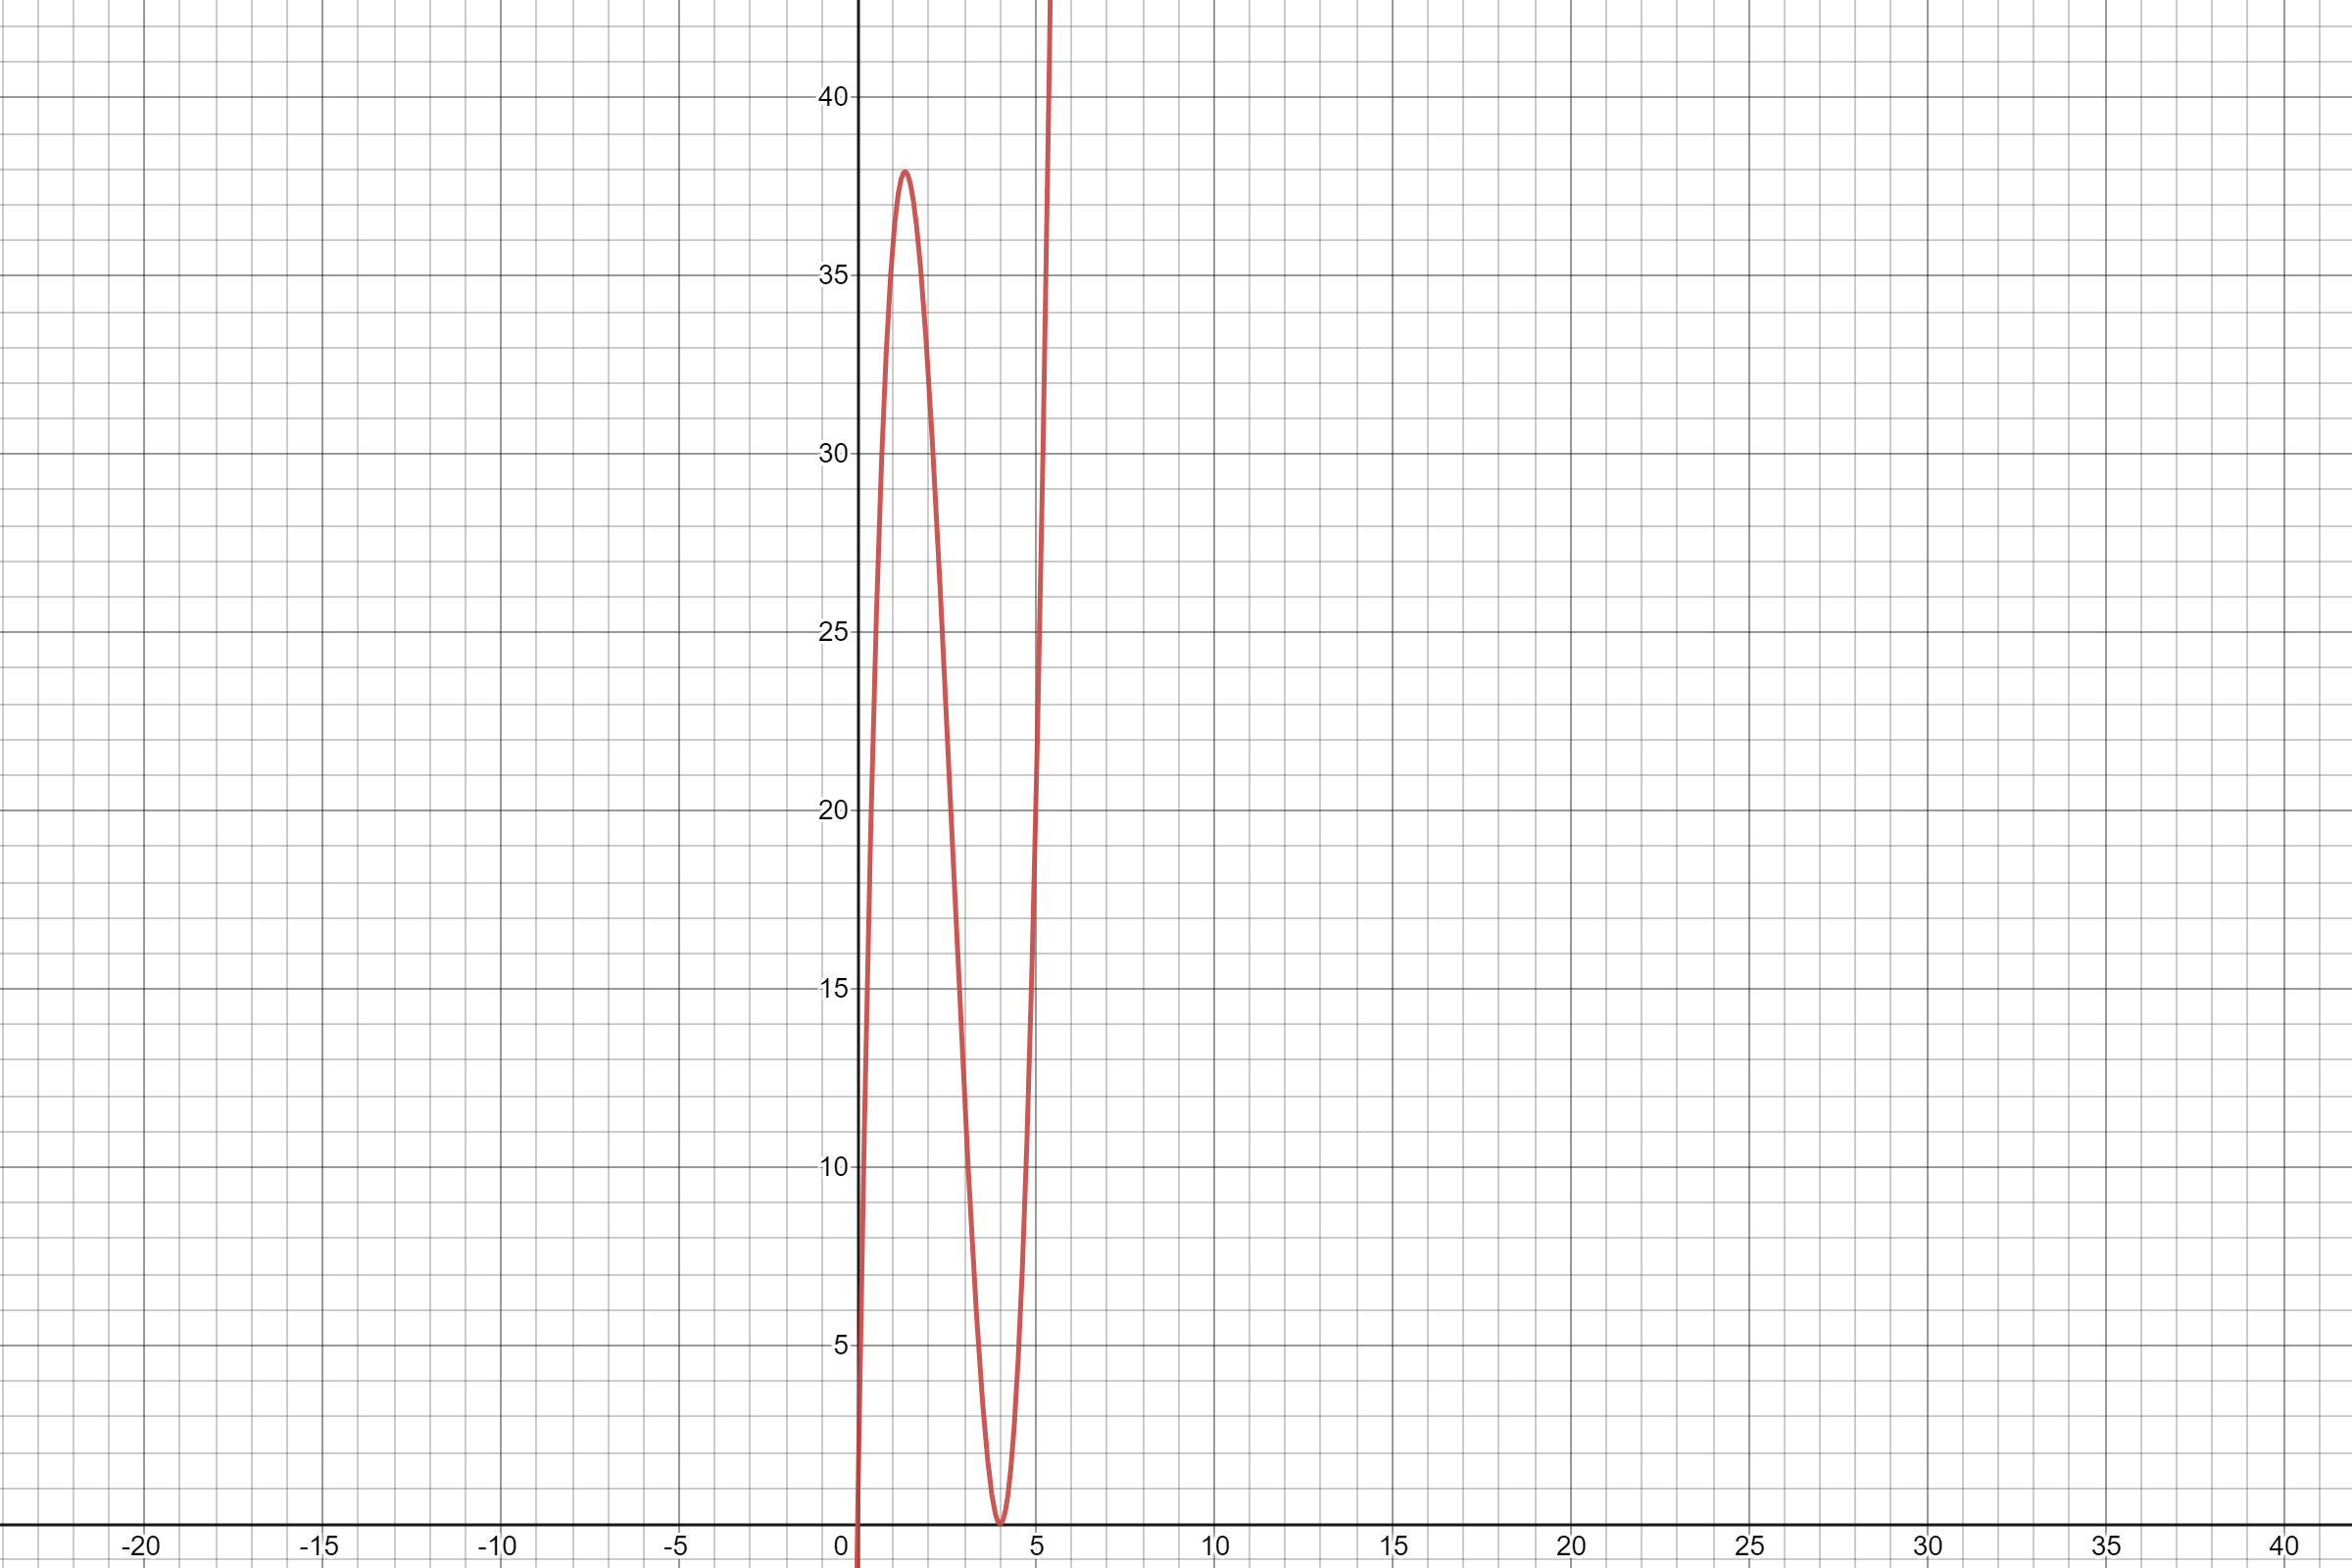
\includegraphics[scale = 0.1]{poly}\\
\\We could also determine what the value of x would need to be at in order to maximize the volume of the box.
\\First we would need to find the domain of the polynomial.
Recall
$${V(x)=l.w.h}$$
$${V(x)=(8-2x)(8-2x)x}$$
We Know that each side of the box has to be greater than zero otherwise it would mean that we are not taking anything from the cardboard, but at the same time these sides have to be less than the original length or width of the cardboard.\\
This can be expressed as
$${0<8-2x}$$
$${-8<-2x}$$
$${4 > x}$$
So what this means is that for you to cut out of the card board and construct a box of Volume v, 
$${0 < x < 4 }$$

THe graph of ${V(x) =64x-32x^2+4x^3}$ can be used to estimate the maximum value of the volume, confined to the values of x within the domain, i.e ${0 < x < 4 }$.\\

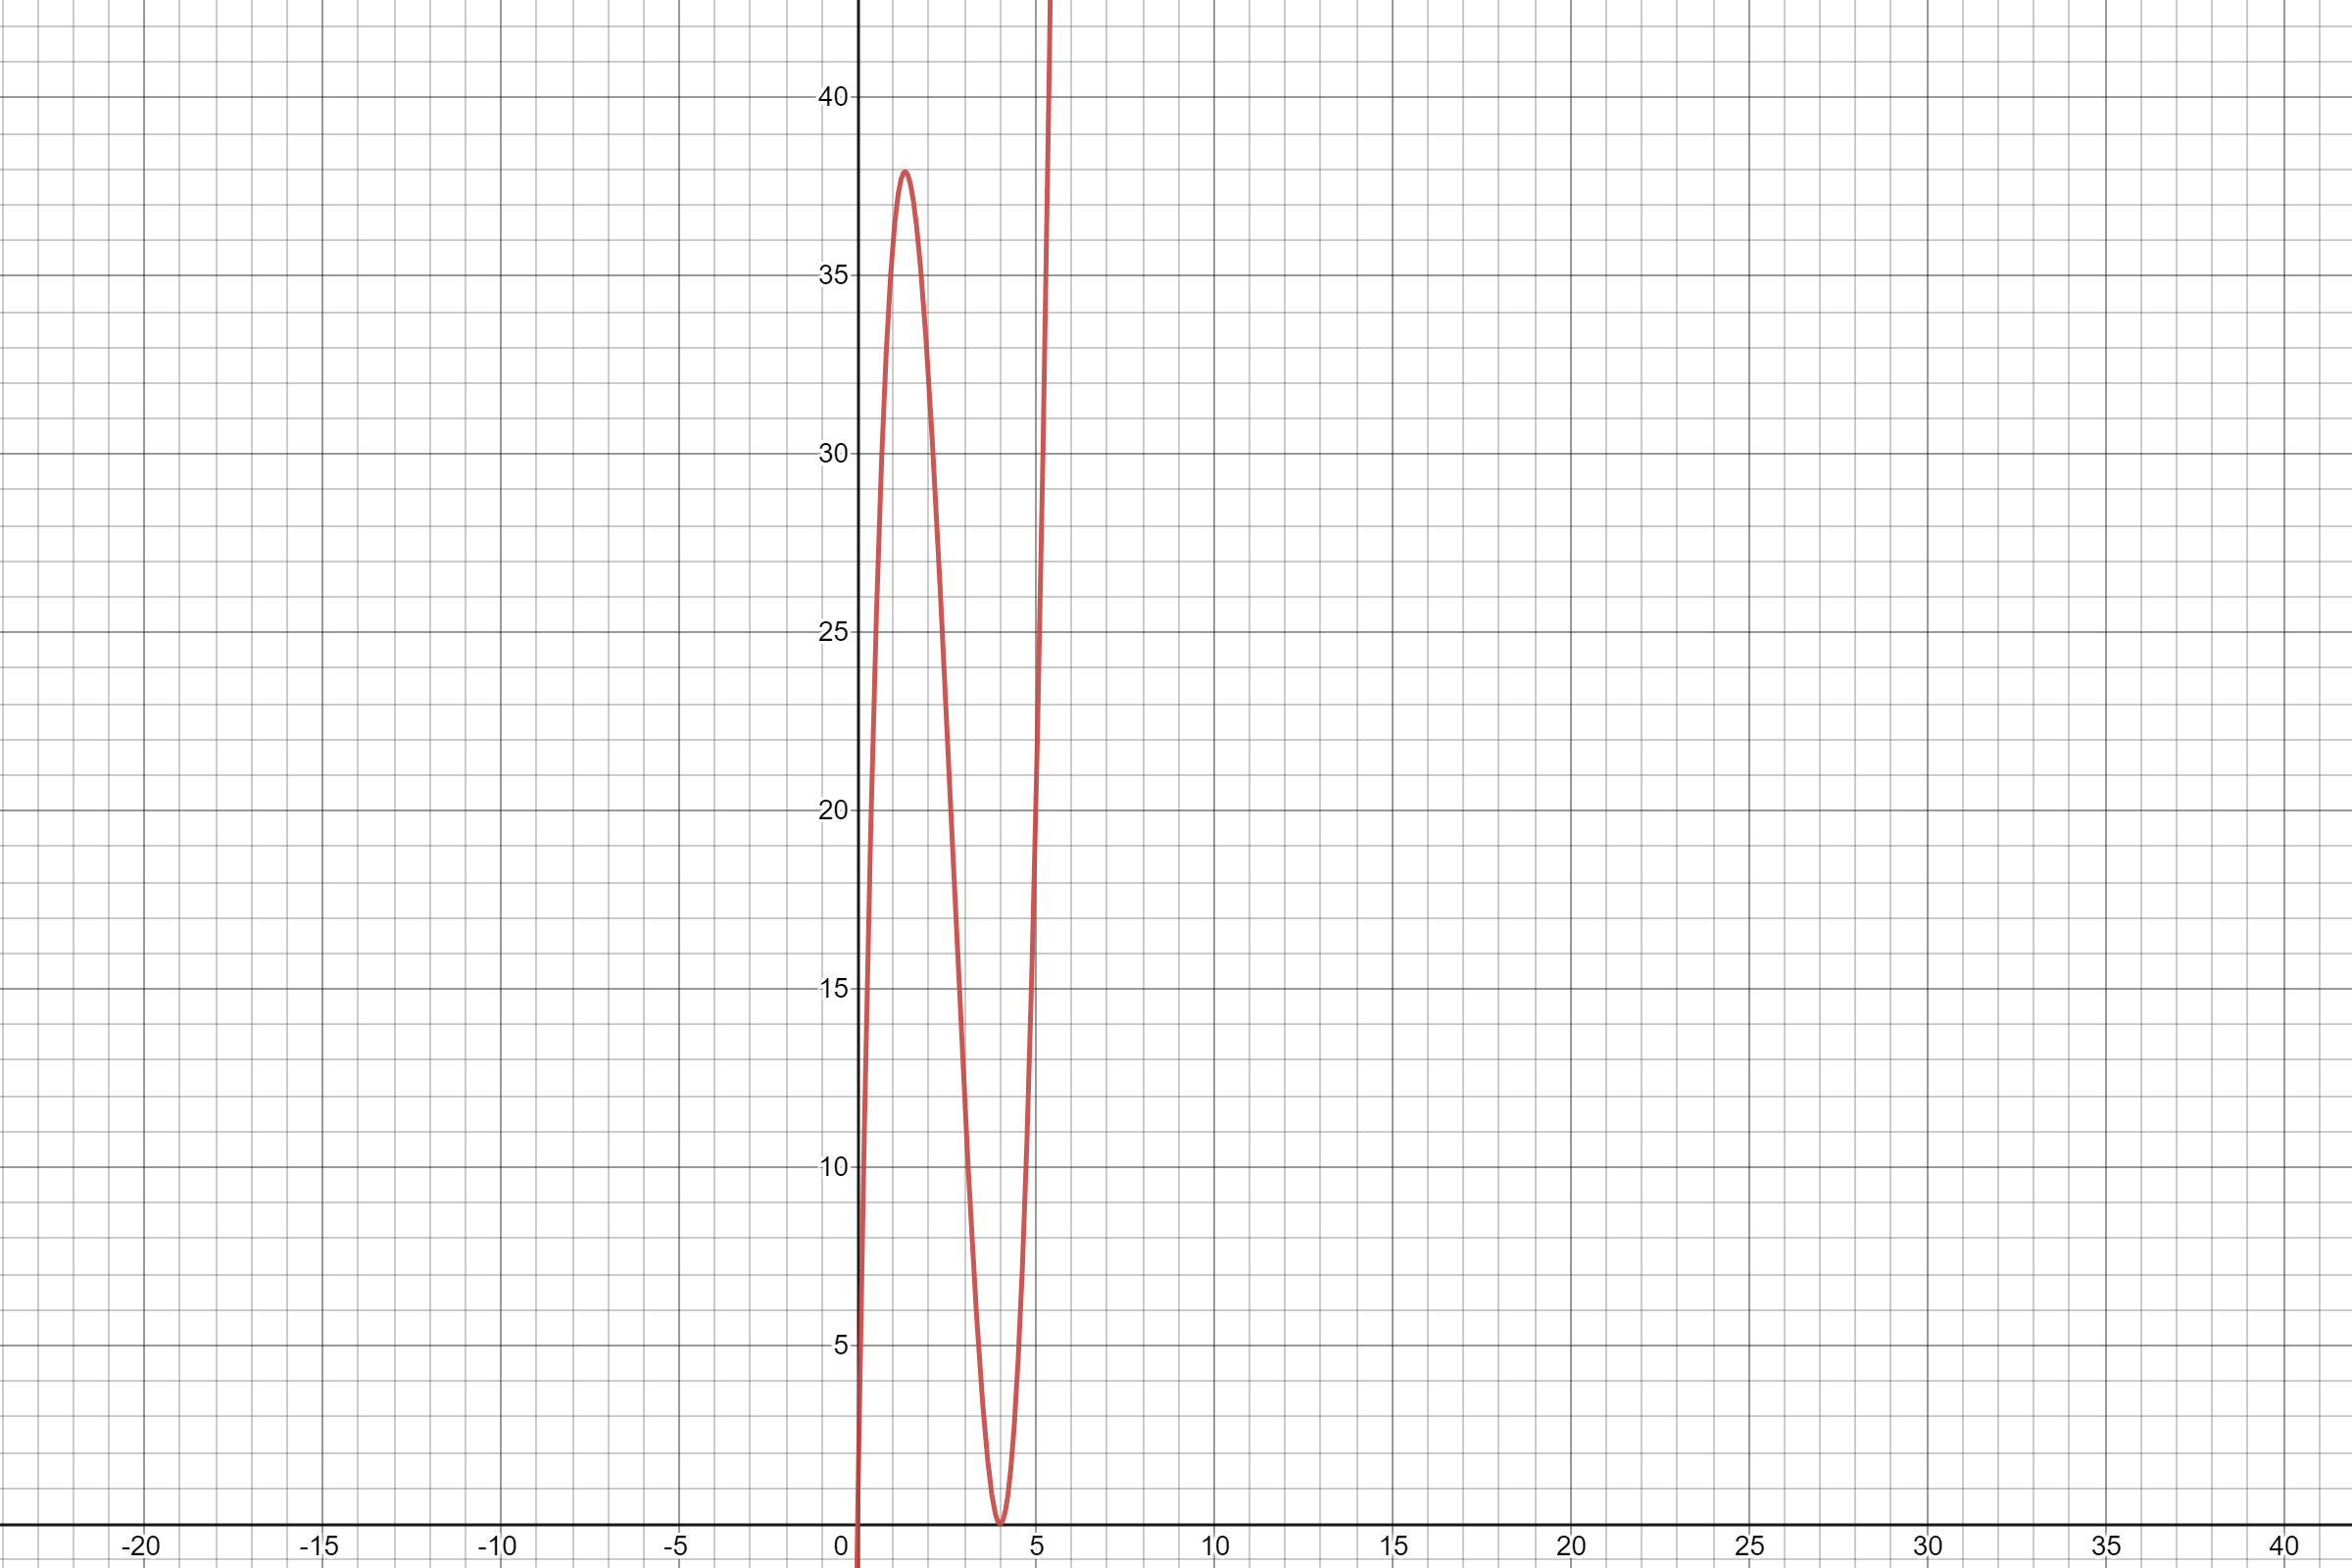
\includegraphics[scale = 0.1]{poly}\\
\\From the graph for the domain [0, 4]. The estimate of the maximum value when zoomed in is ${37.926 inch^3}$ and this occurs when the square corners are about ${1.333 inches}$ on each side.

So Therefore we can say the value of x for which the box would be at the maximum volume is when x is 1.333 inches





\section*{References}
Abramson, J. (2017). \textit{Algebra and trigonometry}. OpenStax, TX: Rice University. Retrieved
from https://openstax.org/details/books/algebra-and-trigonometry\\
\\\textit{Chegg.com.} (2016, March 28). Chegg. https://www.chegg.com/homework-help/questions-and-answers/company-going-make-open-topped-boxes-14-18-inch-rectangles-cardboard-cutting-squares-corne-q11628749
\end{document}
